\chapter{Anhang}



\section{Projektorganisation}



\section{Persönliche Berichte}

\subsection{Florian Bentele}


\subsection{Patrizia Heer}

\subsection{Simon Stäheli}

\section{Anforderungen TourLive Server}
\label{sec:tourliveusecase}
\subsection{Live Stream}
Auf der Webseite werden Bilder von den Aufnahmegeräten zum aktuellen Zeitpunkt angezeigt. Auf den Bildern ist zu erkennen, wann dieses erstellt wurde. Das Bild kann zusätzlich vergrössert werden. Je nach Einstellung werden stehende Bilder (wie in Abbildung 1) oder fliessende Bilder (Videos) übertragen
\begin{figure}[H]
	\centering
	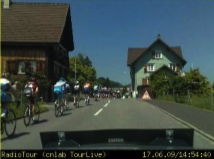
\includegraphics[height=60mm]{images/tourliveaufnahme.png}
	\caption{Aufnahme aus dem Fahrzeug}
\end{figure}

\subsection{Streckenprofil}
Der Verlauf der Strecke wird in einem Streckenprofil dargestellt. Die Position der Aufnahmegeräte wird mit verschiedenen Farben aufgezeichnet, das Streckenprofil an sich ist statisch und beinhaltet zusätzliche Renn-Informationen wie z.B. Sprints oder Passhöhen. Die Zusatzinformationen und Profildaten werden von Bildern, GPS-Daten und/oder der Marschtabelle übernommen.
\begin{figure}[H]
	\centering
	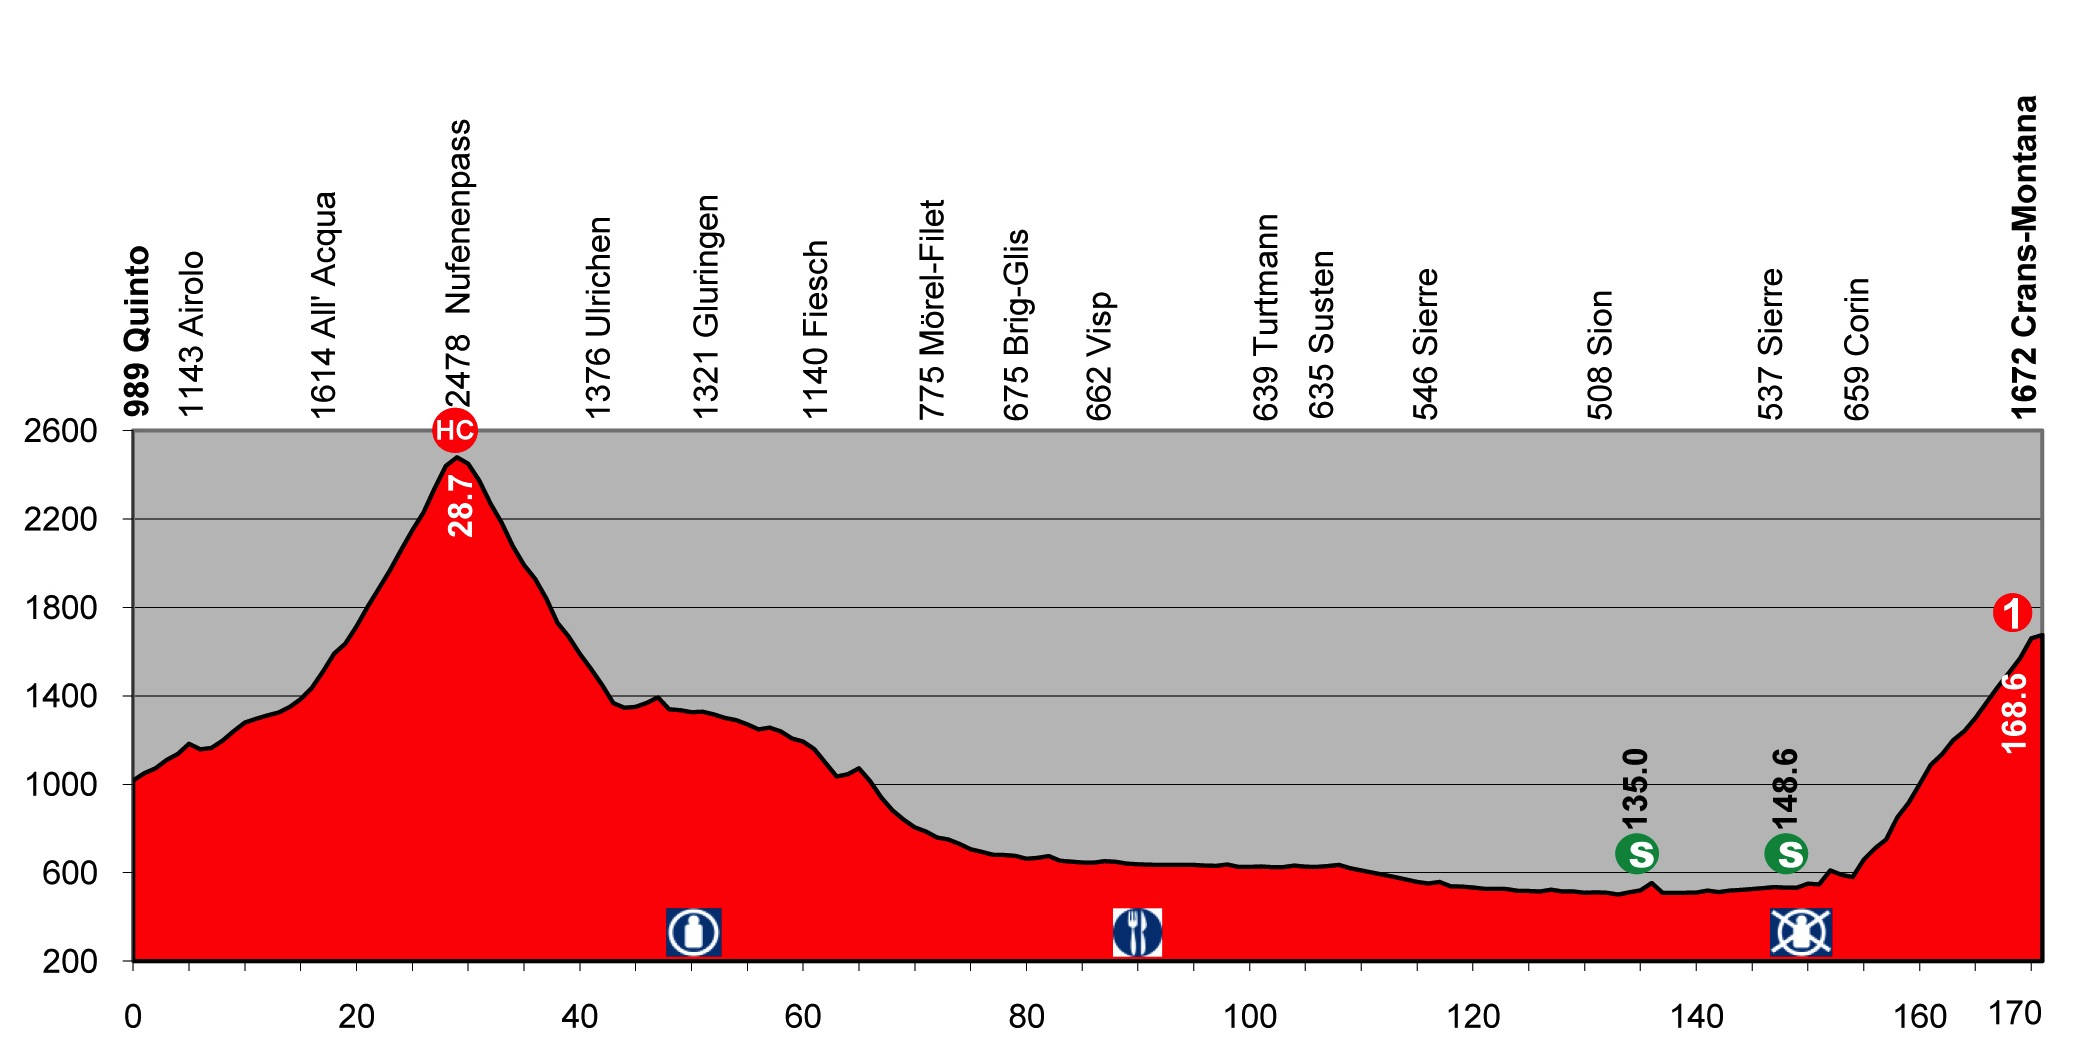
\includegraphics[width=130mm]{images/streckenprofil.jpg}
	\caption{Streckenprofil aus der Tour de Suisse 2013\footnote{Bildquelle: \url{http://tourdesuisse.ch}, Aufgerufen am 08.05.2013}}
\end{figure}

\subsection{Abstände}
Jedes Aufnahmegerät zeichnet unter anderem die aktuelle Geschwindigkeit auf, diese wird wie in Abbildung 3 dargestellt. Der Server versucht zusätzlich die Distanz zwischen den Geräten zu berechnen und zeigt diese zusammen mit dem zeitlichen Rückstand an. Der TourSpeaker kann zusätzlich den Abstand in der Figur überschreiben, sofern diese Daten aktueller sind
\begin{figure}[H]
	\centering
	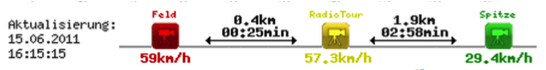
\includegraphics[width=130mm]{images/abstaende.png}
	\caption{Abstände zwischen den Aufnahmesystemen}
\end{figure}

\subsection{Rennsituation}
Die gegenwärtige Rennsituation wird grafisch dargestellt, bei kleineren (Verfolger-) Gruppen werden die Fahrer namentlich aufgelistet, beim Feld wird nur die gesamte Anzahl Fahrer angezeigt. Der Vorsprung bzw. Rückstand ist bei allen Gruppen relativ zur Spitze angegeben. Zusätzlich wird der letzte Wert ebenfalls angegeben, um eine allfällige Tendenz feststellen zu können.
\begin{figure}[H]
	\centering
	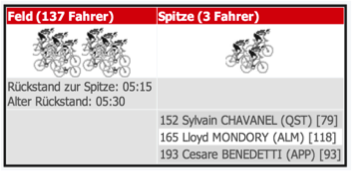
\includegraphics[width=80mm]{images/rennsituation.png}
	\caption{Die aktuelle Rennsituation dargestellt}
\end{figure}
\subsection{Ranglisten}
Aus der aktuellen Rennsituation lässt sich eine virtuelle (Live) Rangliste bestimmen. Diese Rangliste wiederspiegelt den aktuellen Stand im Rennen, kann beliebig sortiert werden und beinhaltet die folgenden Spalten:
\begin{itemize}
\item Rang
\item Startnummer
\item Fahrername
\item Team
\item Land
\item Rückstand zur Spitze
\end{itemize}
Die offiziellen Ranglisten werden von DataSport / Festina / Matsport bezogen.
\subsection{Kartenausschnitt}
Auf einem Kartenausschnitt wird die zurückgelegte Strecke eingezeichnet, die Positionen der Aufnahmegeräte werden auf der Karte farblich verschieden dargestellt. Die Farben entsprechen den anderen Elementen (siehe Abstände und Stream). Neben Google Maps sollen auch andere Karten-APIs verwendet werden könne
\begin{figure}[H]
	\centering
	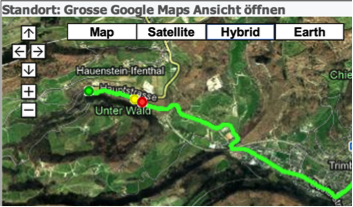
\includegraphics[width=100mm]{images/kartenausschnitt.png}
	\caption{Die Positionen der Aufnahmegeräte}
\end{figure}
\subsection{Live Ticker}
Eine externe Person kann über ein Webinterface einen Live Ticker führen und Ereignisse während dem Rennen erfassen, diese werden dann sofort auf der Webseite dargestellt.
\subsection{Replay}
Das gesamte Rennen wird aufgezeichnet und kann später in Echtzeit oder im Schnelldurchlauf mit verschiedenen Geschwindigkeiten wiedergegeben werden. Je nach Rennen existieren mehrere Etappen, diese können dann einzeln ausgewählt werden. Die vergangenen Rennen können nach Jahr und Event sortiert und ausgewählt werden.
\subsection{Werbebanner}
Auf der Webseite wird ein Bereich definiert, in welchen Werbebanner dargestellt werden. Diese können in den Einstellungen ein und ausgeschaltet werden.
\subsection{Mobile Version}
Die Webseite soll auch auf Tablets und Smartphones sämtliche Informationen darstellen können. Dabei wird der Ansatz des Responsive Web Design verfolgt wobei die Clients die Webseite entsprechend ihrer Bildschirmgrösse rendern.
\begin{figure}[H]
	\centering 
	
\includegraphics[width=80mm]{images/responsive.png}
	\caption{Die Darstellung der Webseite auf die Anzeigegrösse angepasst\footnote{Bildquelle:\url{http://johnpolacek.github.com/scrolldeck.js/decks/responsive/img/responsive_web_design.png}, Aufgerufen am 08.05.2013}}
\end{figure}
\subsection{Rennstandort (Marschtabelle)}
Die Besucher der TourLive Webseite können aufgrund Ihres aktuellen Standortes bestimmen, wann die Spitze am jeweiligen Ort eintreffen wird. Der Standort wird durch die Browser Geolocation API ermittelt damit kann dann die Distanz zur Spitze berechnet werden und aufgrund der Durchschnittsgeschwindigkeit den ungefähren Ankunftszeitpunkt.
Die ungefähren Ankunftszeiten gehen auch aus der Marschtabelle hervor. Diese lässt sich ebenfalls anzeigen.

\subsection{Abstandsentwicklung}
Die verschiedenen Aufnahmesysteme können sich unter Umständen weit voneinander entfernen. Die Entwicklung dieses Abstandes während des Rennen bietet für die Radsport-Kenner ein gutes Bild, wie sich das Feld verändert.
\begin{figure}[H]
	\centering
	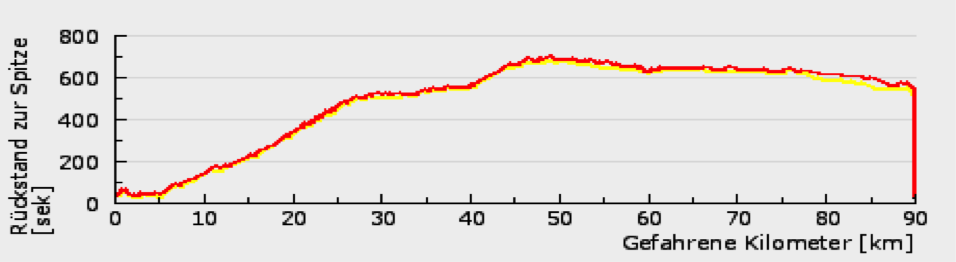
\includegraphics[width=100mm]{images/abstandsentwicklung.png}
	\caption{Abstandsentwicklung nach Rennkilometer in Sekunden}
\end{figure}

\subsection{Public API}
Sämtliche Grafiken und Daten, welche auf der Webseite angezeigt werden, können auch einzeln über eine festgelegte Schnittstelle als JSON empfangen werden. Dies ermöglicht die Entwicklung von beliebigen Anwendungen durch Dritte. Den Zugang zur öffentlichen Schnittstelle wird durch einen API Key ermöglicht, einen solchen Key erhält, wer sich als Entwickler bei TourLive registriert; dadurch kann die Nutzung überwacht und allenfalls eingeschränkt werden.
\subsection{Input API}
Die aktuelle Rennsituation sowie weitere Informationen zum Rennen werden durch mehrere Android Geräte erfasst. Die Aufnahmegeräte senden sämtliche Informationen via JSON an die Serverschnittstelle. 
\\
Weiter werden Daten direkt vom RadioTour Speaker empfangen, diese liefern vor allem Informationen zur Situation im Rennfeld, wie viele Fahrer in welcher Formation fahren.
\subsection{Nutzungsstatisktik}
Über die Nutzung von TourLive wird eine Statistik geführt. Dabei wird auf eine bestehendes Web Analytics System zurückgegriffen, dieses System ist nicht Bestandteil der Arbeit es wird dabei auf Piwik oder Google verwendet.

\section{Evaluation Webframework}
\label{sec:evaluationwebframework}
\subsection{Kriterienkatalog}
Zwingende Kriterien
\begin{itemize}
\item Open Source Software, keine Lizenzgebühren
\item Beispiel- und Referenzprojekte vorhanden
\item Hohe Performance und stabile Verfügbarkeit auch bei hoher Auslastung
\item Skalierbar für mehrere Rennen und Etappen
\item Datenbankanbindung an \gls{mariadb}
\item Weiterentwicklung durch cnlab AG muss möglich sein
\end{itemize}
Optionale, gewünschte Anforderungen
\begin{itemize}
\item Vorkenntnisse in der betreffenden Programmiersprache
\item Gleiche Technologie für API, Webseite und Datenverarbeitung
\item Umfangreiche Dokumentation und Tutorials (Community\footnote{Die Community ist die Verbreitung einer Technologie sowie die Hilfsbereitschaft in Foren und Portalen. Dies ist äusserts schwierig zu beurteilen und kann sich auch schnell ändern.})
\end{itemize}
\subsection{Mögliche Lösungen}
\subsubsection{Django}
Auf Python basiertes Webframework. Wird eingesetzt bei berühmten Webseiten wie z.B. Pinterest, Instagram und The Washington Post.  Django beinhaltet einen OR Mapper, Templates zur Darstellung und einen URL Dispatcher als Controller.
\subsubsection{Spring MVC}
Spring MVC ist ein Framework für die Erstellung von Webprojekten. Es basiert auf Java Technologien und fördert Dependency Injection  und aspektorientierte Programmierung .
\subsubsection{JavaServer Faces}
JSF ist ein Framework-Standard für Webapplikationen in Java. Es verwendet die Java Servlet Technologie und benötigt einen Servlet Container für den Betrieb. Mit JSF können Komponenten für User Interfaces einfach in Webseiten eingebaut werden. 
\subsubsection{Symfony}
Symfony ist ein Open Source PHP Webframework und verfolgt das MVC Pattern. Die Zuordnung der Models geschieht dabei über die Namensgleichheit in Singular und Plural und nicht über Konfigurationsdateien (convention over configuration). Weiter können durch Konsolenapplikationen Anwendungen generiert werden.
\subsubsection{Ruby on Rails}
Rails ist ein Webframework geschrieben in Ruby, es ist geprägt von den Prinzipien „don’t repeate yourself“ und „convention over configuration“. Ruby on Rails besteht aus fünf Modulen, jedes dieser Module übernimmt gewisse Funktionen, so z.B. der Action Mailer versendet und empfängt E-Mails.
\subsection{Nutzwertanalyse}
\begin{figure}[H]
	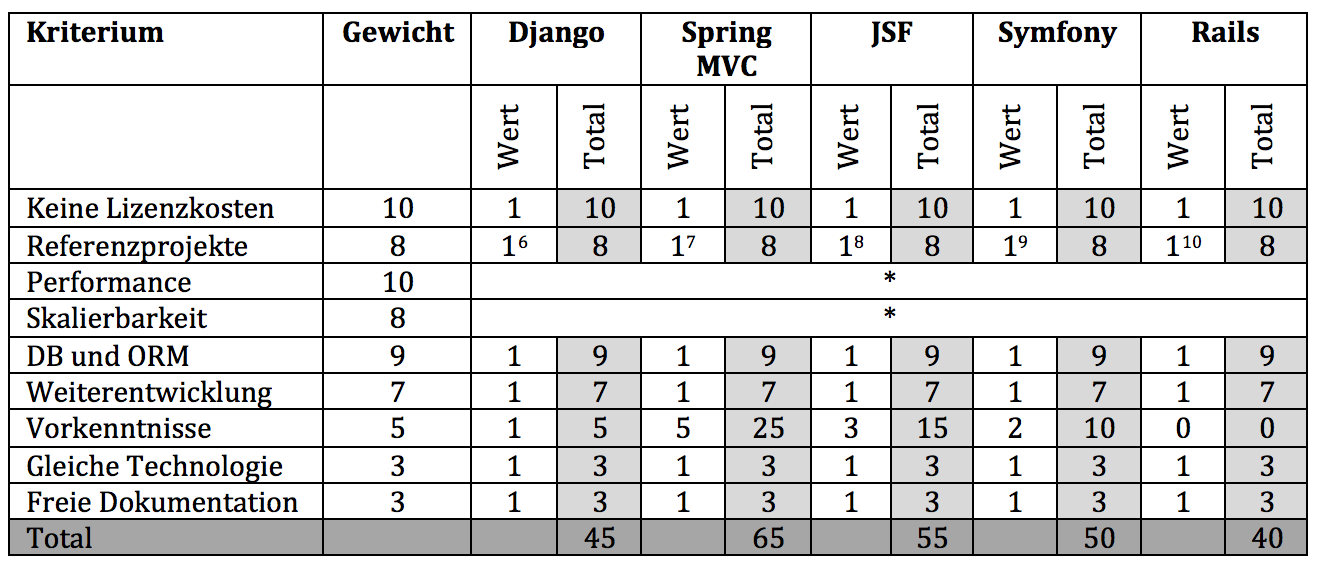
\includegraphics[width=130mm]{images/nutzwertanalyse.png}
	\caption{Nutzwertanalyse}
\end{figure}
\subsubsection{Erläuterung zu Performance und Skalierbarkeit}
Bezüglich der Performance gibt es verschiedene Ansichten zu den verschiedenen Frameworks. Da es aber zu allen obigen Frameworks grosse Projekte gibt, kann davon ausgegangen werden, dass die Performance und Skalierbarkeit für das TourLive Projekt ausreicht.
\subsubsection{Erläuterung zur Gewichtung der Kriterien}
Die verschiedenen Kriterien wurden in einer Skala von 1 – 10 Gewichtet wobei 10 das wichtigste Kriterium darstellt. Gemäss cnlab AG dürfen für das Framework keine Lizenzkosten anfallen und die Webseite muss auch unter Last stabil verfügbar sein. Daher werden diese beiden Kriterien mit dem höchsten Gewicht 10 versehen.
Da das System einen stark wachsenden Datenbestand haben wird, ist die Implementation von Datenbanken ebenfalls von hoher Bedeutung. Referenzprojekte dienen als Beweis für die Skalierbarkeit und die Performance des jeweiligen Frameworks.
Für die Studierenden ist der Zugang zu freier Dokumentation sowie Vorkenntnisse relevant jedoch nicht zwingend erforderlich. Wünschenswert ist ebenfalls, dass für das gesamte Webprojekt dasselbe Framework verwendet werden kann. Diese Punkte werden daher mit den Gewichten 3-5 bewertet.
\subsubsection{DB und ORM}
Ruby on Rails verfolgt das Ziel möglichst abstrakt mit Datenbanken zu arbeiten und kann deshalb problemlos mit verschiedenen Datenbanksystemen arbeiten. Gleichwohl ist der Ansatz bei Django, dort werden verschiedene Datenbankadapter zur Verfügung gestellt. Auch Spring arbeitet z.B. mit Hibernate als ORM problemlos mit verschiedenen Datenbanken.
\subsubsection{Weiterentwicklung durch cnlab AG}
Nach Abschluss der Arbeit wird das Projekt durch die cnlab weiter entwickelt. Daher muss bei der Auswahl des Frameworks darauf geachtet werden, dass eine weitere Entwicklung möglich ist.
\subsubsection{Schlussfolgerungen}
Da die Frameworks sehr ähnliche Ansätze verfolgen und aktuell eine grosse Entwicklergemeinschaft geniessen, sind die Unterschiede, abgesehen von der Programmiersprache welche als Grundlage dient, sehr klein. Entscheidend sind schliesslich die Vorkenntnisse: Java diejenige, für die bereits das grösste Vorwissen besteht. Daher sind für die engere Wahl die beiden Lösungen Spring MVC und JSF im rennen. Da wir in einer kleinen Projektarbeit bereits mit JSF gearbeitet haben möchten wir nach unseren eher negativen  Erfahrungen damit von einer Entwicklung mit JSF absehen und auf das Spring MVC Framework setzen.

\section{Designentscheid}


\section{Werzeuge und Entwicklungsumgebung}
Für die drei Teilprojekte TourLive Server, DeviceManagement Server und Aufnahmesystem wurde jeweils die Java Programmiersprache verwendet. Dennoch gibt es Unterschiede bei den Entwicklungsumgebungen, diese sind im folgenden Abschnitt erläutert.
\subsection{TourLive Server}
\begin{itemize}
\item Entwicklungsumgebung: Spring Tool Suite (STS), basierend auf Eclipse, \url{http://www.springsource.org/sts}
\item Framework: Spring MVC, Java Webframework, \url{http://www.springsource.org/}
\item Mockups: Balsamiq Mockup für erste Entwürfe, \url{http://www.balsamiq.com/}
\item Versionierungssystem: git, \url{http://git-scm.com/}
\end{itemize}

\subsection{DeviceManagement Server}
Java

\subsection{Aufnahmesystem}
Android Java

\subsection{Projektmanagement und weiteres}
Zeitplan und Taskmanagement: Excel und Redmine
Vorgehensmodell: angepasstes RUP
Testing: Prototypen z.T. im Liveumfeld, JUnit
Dokumentation: LaTex für diesen Bericht und Word für Protokolle

\section{Plakat}
<<hier kommt das Plakat>>

\section{Developer Guide}
Installationsanleitung für die weitere Entwicklung.


\section{Zugänge}
Die Coderepositories sind auf Github öffentlich zugänglich. Zugang zum Server... 

\section{Kontaktadressen}
\subsubsection{Die Studierenden}

Simon Stäheli\\
Im Langacher 21\\
8805 Richterswil\\
sstaehel@hsr.ch\\

Patrizia Heer\\
Friedbergstrasse 13b\\
8512 Thundorf\\
pheer@hsr.ch\\

Florian Bentele\\
Teufener Strasse 113\\
9000 St. Gallen\\
+41 78 883 68 65\\
florian@bentele.me\\

Der betreuende Professor\\
Prof. Dr. Peter Heinzman, cnlab AG\\
Obere Bahnhofstrasse 32b\\
8640 Rapperswil\\
+41 79 243 04 61\\
peter.heinzmann@cnlab.ch\\

Der Industriepartner\\
Lukas Frey, cnlab AG\\
Obere Bahnhofstrasse 32b\\
8640 Rapperswil\\
+41 55 214 33 44\\
lukas.frey@cnlab.ch

\section{Inhaltsverzeichnis der CD}
.\\
|-01Dokumente-cnlab\\
||Alte Logos\\
||logo.png\\
|-02Protokolle\\
|--01Protokoll.doc\\
|--02Protokoll.doc\\

